% Draft/preview of TikZ versions of Figs 1.1 and 1.2 for approval.
% Standalone: build with  xelatex Chap1_figures_draft.tex  (or pdflatex).
% Manual axonometric projection via a custom tikz x/y/z basis, so nothing
% beyond plain tikz is needed -> the code drops straight into the book.
%
% Colour convention (axes stay black, per request):
%   position vector r : blue
%   Cartesian basis e_x,e_y,e_z : red
%   spherical basis  e_r (red), e_theta (green), e_phi (orange)
%   dashed construction lines/arcs : gray ; angle arcs : black
\documentclass[11pt]{article}
\usepackage[a4paper,margin=2cm]{geometry}
\usepackage{amsmath}
\usepackage{tikz}
\usetikzlibrary{arrows.meta}

% shared axonometric basis: x -> down-left (foreshortened), y -> right, z -> up
\tikzset{
  axo/.style={x={(-0.72cm,-0.46cm)}, y={(1cm,0cm)}, z={(0cm,1cm)}},
  axis/.style={black, thick, -{Latex[length=2.4mm]}},
  rvec/.style={blue!70!black, ultra thick, -{Latex[length=2.8mm]}},
  bvec/.style={red!80!black, ultra thick, -{Latex[length=2.4mm]}},
  cdash/.style={black!45, very thick,dashed},
  rdash/.style={red!80!black, very thick,dashed},
  arc/.style={black, thin},
  % extra styles for Fig 1.3 (Euler-rotation stages)
  nvec/.style={blue!70!black, very thick, -{Latex[length=2.4mm]}},   % axis after this stage's rotation
  gvec/.style={green!55!black, very thick, -{Latex[length=2.4mm]}},  % final (primed) axes
  odash/.style={black!55, thick, dashed},                            % axis/plane from a previous stage
  bdash/.style={blue!60!black, thick, dashed},                       % "before" axes in stage (c)
  disk/.style={fill=black!7, draw=black!55, thin},                   % reference (xy) plane
  tdisk/.style={fill=blue!8, draw=blue!55, thin},                    % tilted plane
  rota/.style={black, thick, -{Latex[length=2.2mm]}},                % rotation-sense arc
}

\begin{document}
\thispagestyle{empty}
\begin{center}\large\bfseries Chapter 1 figures --- TikZ draft for approval\end{center}
\vspace{1em}

%======================================================================
% FIG 1.1  Cartesian coordinate system
%======================================================================
\begin{center}
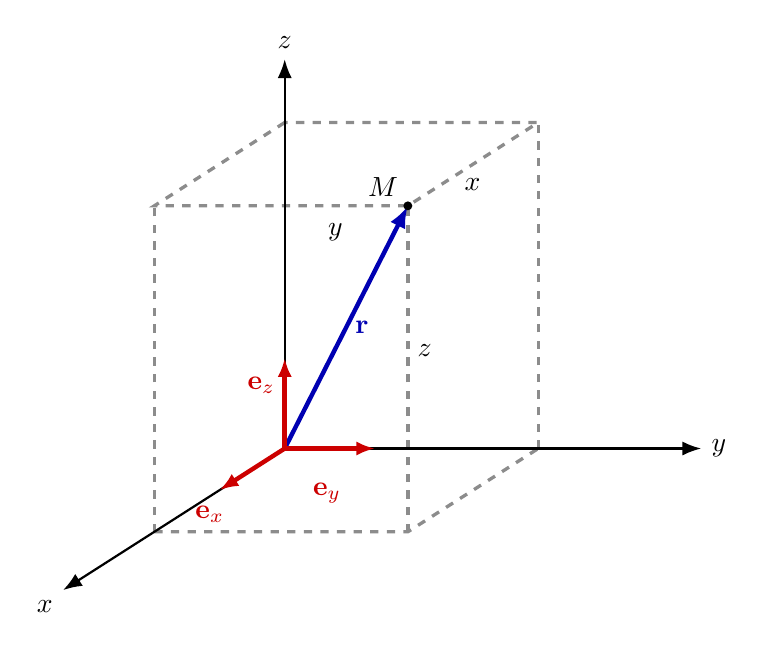
\begin{tikzpicture}[axo, scale=1.15]
  % --- dashed projection box (corners of the parallelepiped O..M) ---
  % O=(0,0,0) A=(2,0,0) B=(0,2.8,0) C=(0,0,3.6) Q=(2,2.8,0)
  % D=(2,0,3.6) E=(0,2.8,3.6) M=(2,2.8,3.6)
  \draw[cdash] (2,0,0)--(2,2.8,0)--(0,2.8,0);          % A-Q-B (bottom, front)
  \draw[cdash] (0,0,3.6)--(2,0,3.6)--(2,2.8,3.6)--(0,2.8,3.6)--(0,0,3.6); % top face
  \draw[cdash] (2,0,0)--(2,0,3.6);                     % A-D
  \draw[cdash] (2,2.8,0)--(2,2.8,3.6);                 % Q-M (vertical, labelled z)
  \draw[cdash] (0,2.8,0)--(0,2.8,3.6);                 % B-E

  % --- axes (black) ---
  \draw[axis] (0,0,0)--(3.4,0,0) node[below left]{$x$};
  \draw[axis] (0,0,0)--(0,4.6,0) node[right]{$y$};
  \draw[axis] (0,0,0)--(0,0,4.3) node[above]{$z$};

  % --- position vector r to M ---
  \draw[rvec] (0,0,0)--(2,2.8,3.6);
  \node[blue!70!black] at (0.9,1.5,1.75) {$\mathbf{r}$};
  \fill (2,2.8,3.6) circle (1.4pt);
  \node[above left] at (2,2.8,3.6) {$M$};

  % --- box edge dimension labels ---
  \node[right] at (2,2.8,2) {$z$};
  \node[above] at (2,2,3.1) {$y$};
  \node[above right] at (1.0,2.6,3.2) {$x$};

  % --- Cartesian basis vectors (red) ---
  \draw[bvec] (0,0,0)--(1,0,0);  \node[red!80!black,below]  at (1.15,0,0) {$\mathbf{e}_x$};
  \draw[bvec] (0,0,0)--(0,1,0);  \node[red!80!black,below]       at (0.6,0.9,0) {$\mathbf{e}_y$};
  \draw[bvec] (0,0,0)--(0,0,1);  \node[red!80!black,left]        at (0,0,0.7) {$\mathbf{e}_z$};
\end{tikzpicture}

\textbf{Fig.~1.1.} Cartesian coordinate system.
\end{center}

\vspace{2.5em}

%======================================================================
% FIG 1.2  Spherical (polar) coordinate system
%======================================================================
\begin{center}
\begin{tikzpicture}[axo, scale=1.15]
  % sphere radius R=4, point P at theta=40 deg, phi=50 deg
  % P=(1.653,1.970,3.064)  Q=(1.653,1.970,0)  E=(2.571,3.064,0)

  % --- dashed octant arcs on the sphere ---
  \draw[cdash] plot[variable=\t,domain=0:90,samples=60] ({4*sin(\t)},0,{4*cos(\t)}); % xz meridian
  \draw[cdash] plot[variable=\t,domain=0:90,samples=60] (0,{4*sin(\t)},{4*cos(\t)}); % yz meridian
  \draw[cdash] plot[variable=\t,domain=0:90,samples=60] ({4*cos(\t)},{4*sin(\t)},0); % equator quarter
  % meridian through P (azimuth 50 deg): passes the pole, P and E
  \draw[rdash] plot[variable=\t,domain=0:90,samples=60]
       ({2.571*sin(\t)},{3.064*sin(\t)},{4*cos(\t)});

  % --- drop line P->Q and radius O->Q in the xy-plane ---
  \draw[cdash] (1.653,1.970,3.064)--(1.653,1.970,0);   % P -> Q
  \draw[cdash] (0,0,0)--(1.653,1.970,0);               % O -> Q

  % --- axes (black) ---
  \draw[axis] (0,0,0)--(5,0,0) node[below left]{$x$};
  \draw[axis] (0,0,0)--(0,5.5,0) node[right]{$y$};
  \draw[axis] (0,0,0)--(0,0,5) node[above]{$z$};

  % --- position vector r ---
  \draw[rvec] (0,0,0)--(1.653,1.970,3.064);
  \node[blue!70!black] at (1.25,1.4,2.4) {$\mathbf{r}$};
  \fill (1.653,1.970,3.064) circle (1.4pt);

  % --- angle theta (between z-axis and r), radius 1.1, azimuth 50 ---
  \draw[arc] plot[variable=\t,domain=0:40,samples=30]
       ({1.1*sin(\t)*0.643},{1.1*sin(\t)*0.766},{1.1*cos(\t)});
  \node at (0.42,0.5,1.45) {$\vartheta$};

  % --- angle phi (in xy-plane, from x-axis to OQ), radius 1.0 ---
  \draw[arc] plot[variable=\t,domain=0:50,samples=30] ({1.0*cos(\t)},{1.0*sin(\t)},0);
  \node at (1.3,0.8,0) {$\varphi$};

  % --- local spherical basis at P ---
  \draw[bvec]   (1.653,1.970,3.064)--(2.190,2.610,4.060);
  \node[red!80!black,above]      at (2.19,2.61,4.10) {$\mathbf{e}_r$};
  \draw[bvec] (1.653,1.970,3.064)--(2.293,2.733,2.228);
  \node[red!80!black,right]    at (2.29,2.73,2.20) {$\mathbf{e}_\vartheta$};
  \draw[bvec] (1.653,1.970,3.064)--(0.657,2.806,3.064);
  \node[red!80!black,above]   at (0.66,2.81,3.10) {$\mathbf{e}_\varphi$};
\end{tikzpicture}

\textbf{Fig.~1.2.} Polar (spherical) coordinate system.
\end{center}

\newpage
%======================================================================
% FIG 1.3  Succession of rotations, scheme A  (three Euler stages)
%======================================================================
\begin{center}
\begin{minipage}[t]{0.32\textwidth}\centering
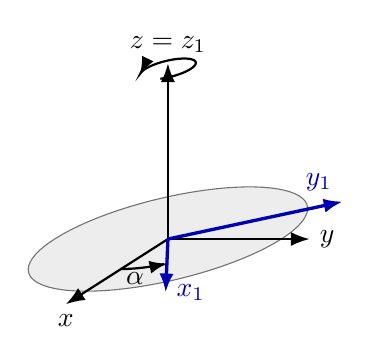
\begin{tikzpicture}[axo, scale=0.72]
  \draw[disk] plot[variable=\t,domain=0:360,samples=80] ({2*cos(\t)},{2*sin(\t)},0)--cycle;
  \draw[axis] (0,0,0)--(2.5,0,0) node[below]{$x$};
  \draw[axis] (0,0,0)--(0,2.5,0) node[right]{$y$};
  \draw[axis] (0,0,0)--(0,0,3.1) node[above]{$z=z_1$};
  \draw[nvec] (0,0,0)--(2.048,1.435,0) node[right]{$x_1$};
  \draw[nvec] (0,0,0)--(-1.435,2.048,0) node[above left]{$y_1$};
  % rotation angle alpha (x -> x1) about z
  \draw[rota] plot[variable=\t,domain=0:35,samples=20] ({1.15*cos(\t)},{1.15*sin(\t)},0);
  \node at (1.5,0.5,0) {$\alpha$};
  % sense of rotation about z
  \draw[rota] plot[variable=\t,domain=20:300,samples=40] ({0.4*cos(\t)},{0.4*sin(\t)},3.0);
\end{tikzpicture}\\[2pt]
(a) rotate about $z$ by $\alpha$
\end{minipage}\hfill
\begin{minipage}[t]{0.32\textwidth}\centering
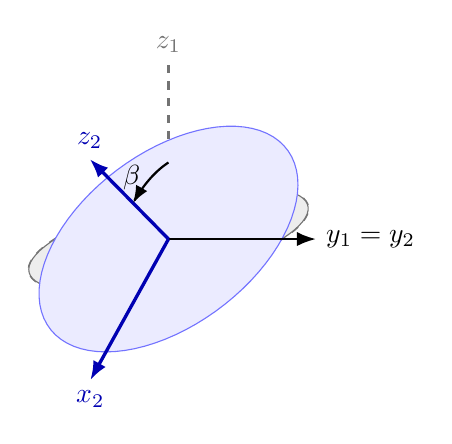
\begin{tikzpicture}[axo, scale=0.72]
  % previous (stage a) plane and vertical axis, as reference
  \draw[odash] plot[variable=\t,domain=0:360,samples=80] ({2*cos(\t)},{2*sin(\t)},0)--cycle;
  \draw[odash] (0,0,0)--(0,0,3.1) node[above]{$z_1$};
  \draw[odash] (0,0,0)--(2.5,0,0) node[below]{$x_1$};
  % tilted plane after rotation about y1 by beta
  \draw[disk] plot[variable=\t,domain=0:360,samples=80] ({2*cos(\t)},{2*sin(\t)},0)--cycle;
  \draw[tdisk] plot[variable=\t,domain=0:360,samples=80]
       ({1.532*cos(\t)},{2*sin(\t)},{-1.286*cos(\t)})--cycle;
  \draw[axis] (0,0,0)--(0,2.6,0) node[right]{$y_1=y_2$};
  \draw[nvec] (0,0,0)--(1.929,0,2.298) node[above]{$z_2$};
  \draw[nvec] (0,0,0)--(1.915,0,-1.608) node[below]{$x_2$};
  % rotation angle beta (z1 -> z2) about y1
  \draw[rota] plot[variable=\t,domain=0:40,samples=20] ({1.35*sin(\t)},0,{1.35*cos(\t)});
  \node at (0.9,0,1.5) {$\beta$};
\end{tikzpicture}\\[2pt]
(b) rotate about $y_1$ by $\beta$
\end{minipage}\hfill
\begin{minipage}[t]{0.32\textwidth}\centering
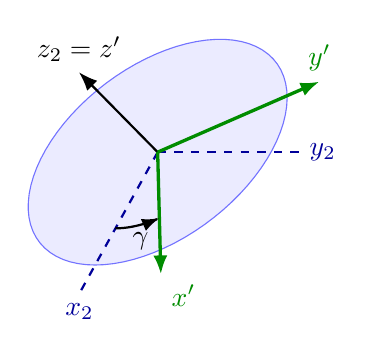
\begin{tikzpicture}[axo, scale=0.72]
  \draw[tdisk] plot[variable=\t,domain=0:360,samples=80]
       ({1.532*cos(\t)},{2*sin(\t)},{-1.286*cos(\t)})--cycle;
  \draw[axis] (0,0,0)--(1.929,0,2.298) node[above]{$z_2=z'$};
  % axes before this stage (dashed)
  \draw[bdash] (0,0,0)--(1.915,0,-1.608) node[below]{$x_2$};
  \draw[bdash] (0,0,0)--(0,2.5,0) node[right]{$y_2$};
  % axes after rotation about z2 by gamma
  \draw[gvec] (0,0,0)--(1.658,1.25,-1.392) node[below right]{$x'$};
  \draw[gvec] (0,0,0)--(-0.957,2.165,0.804) node[above]{$y'$};
  % rotation angle gamma (x2 -> x') about z2
  \draw[rota] plot[variable=\t,domain=0:30,samples=20]
       ({1.35*cos(\t)*0.766},{1.35*sin(\t)},{-1.35*cos(\t)*0.643});
  \node at (1.25,0.6,-1.0) {$\gamma$};
\end{tikzpicture}\\[2pt]
(c) rotate about $z_2=z'$ by $\gamma$
\end{minipage}
\end{center}

\textbf{Fig.~1.3.} Succession of rotations of a coordinate system according to scheme $A$.

\end{document}
